\newpage
\section{Background Knowledge}
This section will first introduce Bayesian Network and Bayesian inference, then, it will introduce logic normal forms, and several other concepts to aid the understanding of the later sections.
    \subsection{Bayesian Network}
    The variable domain in this report refers to finite domains. The definition of the Bayesian network is from \cite{2008-literature-review}\\
    \begin{itemize}
        \item instantiation: An instantiation of a set of Variables \textbf{X} is an assignment to each $X \in$ \textbf{X} of the value within the domain of X.
        \item Joint distribution over \textbf{X} is the probability function F that map the instantiation to the value in [0, 1], The $\Sigma$ F(X) = 1.
        \item factor: factors are functions that can represent in different ways. In bayesian networks, factor is simply the Conditional Probability Tables (CPT).
    \end{itemize}
    \textbf{Bayesian networks} are probabilistic models (G, P) that specify joint probability distributions. G denotes the directed acylic graphs (DAG), and P denotes the set of factors. For each node \textit{X} with random variables $\{x_{1}, ... x_{m}\}$ and its a parents \textit{Y}, there's a conditional probability distribution $P(x_{i}|Y)$. \\
    
    \noindent The joint probability distribution of the Bayesian network: 
    $$P(x_{1}, ... , x_{m}) = \Pi_{i = 1}^{m} P(x_{i}|Y)$$
    $$P(x_{1},.., x_{m}) = \Pi_{i = 1}^{m}P(x_{i}|x_{i - 1}, .. x_{1})$$
    So Bayesian networks assume that given values of parents of a network variable $X$, $X$ is independent of all its other predecessor variables in the graph and it can be written as: $$P(x_{i}|x_{i- 1}, ..., x_{1}) = P(x_{i}|Y)$$
    
    \noindent The Conditional distributions $P(X|Y)$ are obtained as follow:
    $$P(X|Y) = \frac{P(X,Y)}{P(X)}$$
    An example of a Bayesian Network called Asia.net from bnlearn repository is given in Figure 
    
    \begin{figure}
        \centering
        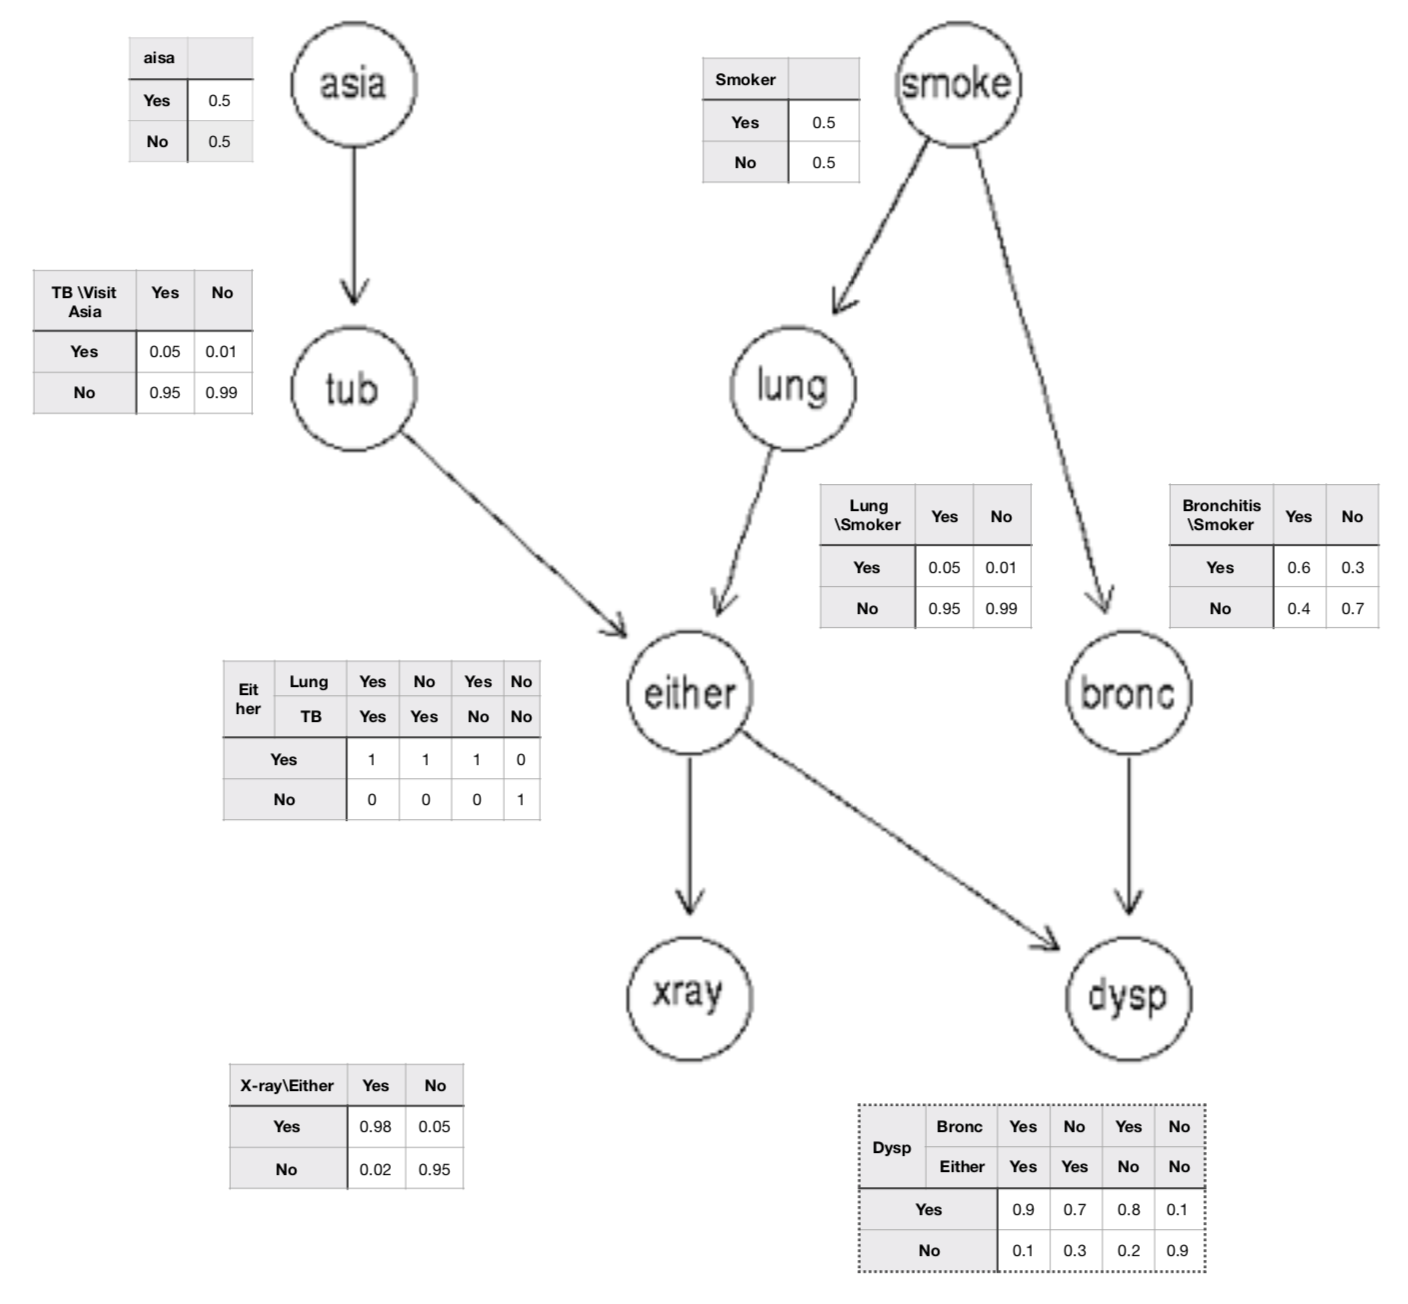
\includegraphics[width = 0.7\textwidth]{pic/full-asia.png}
        \caption{An example Bayesian network Asia.net modeling the toy process of diagnosing lung canber}
        \label{fig:asia-net}
    \end{figure}
    
    \subsection{Exact Bayesian Inference}
    % Given a Joint density for X = $(X_{i}, i \in V)$ of the following form:
    % $$p(u) = \frac{1}{Z} \Pi_{c \in C} \Phi_{c}(u_(c))$$
    % Compute the marginal density of $X_{Q}$:
    % $$p_{q}(v) = \Sigma_{u \in X_{\bar{Q}}} \frac{1}{Z} \Pi_{c \in C} \Phi_{C}(v_{c} \cup u_{c})$$
    Given an Bayesian Network BN over Variables ${X, Y...}$. and probability distributions \textbf{Pr}. There are three reasonable questions to ask regarding the probability distributions:
    \begin{itemize}
        \item What is the most likely instantiation of network variables X given some evidence \textbf{e}
        $$MPE(e) = argmax_{x} Pr(x, e)$$
        \item What is the probability of an evidence \textbf{e}.
        \item What is the assignment y over the complete variables that maximize $P(y|x)$ given an evidence \textbf{x}
    \end{itemize}
    \subsection{Multi\-linear functions}
    A \textit{multi\-linear function} over variables $\Sigma$ is a function
    with the form $t_{1} + t_{2} + ... + t_{n}$ in which each term $t_{i}$ is a product of some distinct variables. \\
    $\Sigma = \lambda_{x}, \lambda_{y}, \lambda_{z}, \theta_{1}, \theta_{2}, \theta_{3}$, an example of muti\-linear function: $f = \lambda_{x}\theta_{1} + \lambda_{y}\theta_{2} + \lambda_{z}\theta_{3}\theta_{2}$\\
    
    \noindent In the project, the idea of CNF encoding of Bayesian networks is to represent the Bayesian network with multi-linear function and then perform the encoding.
    
    \subsection{Normal Forms}
    \textbf{Conjunctive Normal Forms}\\
    
    \noindent In boolean logic, a clause that contains only $\vee$ is called \textbf{disjunctive clause}, and a clause contains only $\wedge$ is called \textbf{Conjunctive clause}.\\
    Conjunctive Normal Forms (also written as clausual normal form) is  the conjunction (\textit{AND}) of one or several clauses, and is a disjunction (\textit{OR}) of literals. An example is given below: $$(p \vee q \vee \neg r) \wedge (\neg q \vee s)$$
    
    \noindent \textbf{Negation Normal Forms}\\
    
    \noindent A formula is in \textbf{negation normal form}  (NNF) if the negation operator is only applied to variables and the only other allowed operators are conjunction (AND) and disjunction (OR).\\
    \newpage
    \noindent \textbf{Decomposability, Determinism Negation Normal Form}\\
    
    \begin{itemize}
        \item \textbf{Decomposibility}: In an NNF, for any two children $node_{i}$ and $node_{j}$, and any node \textit{n} $Variables(node_{i}) \cap Variabes(node_{j}) = \emptyset$.
        \item \textbf{determinism}: In an NNF, for any two children $n_{i} \wedge n_{j}$ is logically inconsistent for any node connected by \textbf{\textit{or}}.
        \item \textbf{Smoothness}: In an NNF, for each disjunction C in the NNF, $C_{1}, ... C_{n}$ mentioens the same variables.
    \end{itemize}
    
    \noindent Three figures of examples are given in \cite{2002language-map} to show these properties, shown in Figure \ref{fig:demo-DDNNF}.
    \begin{figure}
        \centering
        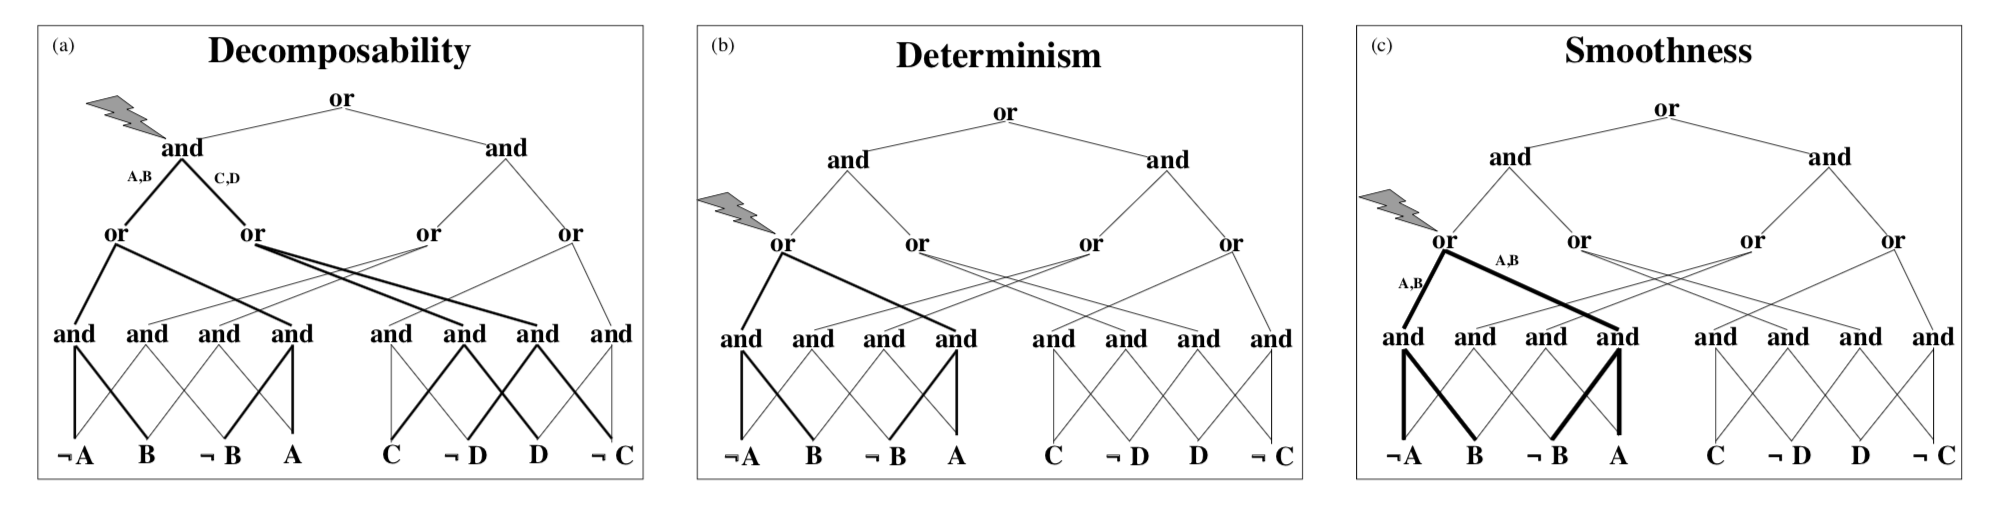
\includegraphics[width = 0.8\textwidth]{pic/DDNNF.png}
        \caption{The example which demonstrate the property of Decomposiblity, Determinism and Smoothness of a NNF given in \cite{2002language-map}}
        \label{fig:demo-DDNNF}
    \end{figure}
    
    \subsection{DPLL}
    Davis–Putnam–Logemann–Loveland (DPLL) algorithm is a complete, backtracking-based search algorithm for deciding the satisfiability of propositional logic formula in conjunctive normal forms \cite{Davis:1960:CPQ:321033.321034}. The algorithm runs by assigning a truth value to a chosen literal to simplify the formula then check satisfiablity recursively.\\ 
    \noindent \textbf{Unit propagation}:\\
    \noindent If a clause contains only one single literal that is not assigned, assign the value that make this literal true.\\
    \noindent \textbf{Pure literal elimination}:\\
    \noindent If a formula contains a propositional variable with only one polarity, remove all the clauses that contains the variable.\\
    
    \noindent The DPLL algorithm is described below based on \cite{DPLLbook}:
    \begin{lstlisting}[mathescape]
    function DPLL($\Phi$)
       if $\Phi$ is a consistent set of literals
           return true;
       if $\Phi$ contains empty clause
           return false;
       for every unit clause {l} in $\Phi$
          $\Phi$ <-  unit-propagate(l, $\Phi$);
       for every literal l that occurs pure in $\Phi$
          $\Phi$  <- pure-literal-assign(l, $\Phi$);
       l gets choose-literal($\Phi$);
       return DPLL($\Phi$ $\wedge$ {l}) or DPLL($\Phi$ $\wedge$ {$\neg$ (l)});
    \end{lstlisting}
    
   
    \subsection{Sensitional Decision Diagram}
    According to \cite{Darwiche:2011:SNC:2283516.2283536}, Sensitional Decision Diagram (SDD) is a Boolean function F(X,Y) which can always be decomposed into the following format:
    $$f(\textbf{X, Y}) = (p_{1}(X) \wedge s_{1}(Y)) \vee (p_{n}(X) \wedge s_{n}(Y)) $$
    The X and Y are disjoint set that $X \wedge Y = \emptyset$ and the decomposition satisfies the \textbf{X-Y partition}. It has been shown in \cite{Darwiche:2011:SNC:2283516.2283536} that it is a traceable representation of Boolean function.
    \textbf{X-Y partition} holds if the decomposition of the boolean function satisfy the following:
    \begin{itemize}
        \item  $\forall$ i, $p_{i} \neq FALSE$;
        \item for $i \neq j$, $p_{i} \wedge p_{j} = FALSE$
        \item $p_{1} \vee ... \vee p_{n} = TRUE$
    \end{itemize}
    
    \subsection{Propositional Model Counting}
    Propositional Model counting is the problem of counting the number of models for a certain propositional formula.\cite{Biere:2009:HSV:1550723-sat-handbook} That is, counting the number of unique assignment that make the formula TRUE. This problem can be solved by exploiting DPLL and local search algorithms.
    
    \subsection{Deterministic Belief network}
    Belief networks which have 0/1 parameters, except possibly for the parameters of root variables, are known as deterministic belief networks.\cite{enc1}
    
    
    